\section{Introduction}
As part of the ongoing study of the structure of nucleons \cite{Avakian:2010ae}  in Hall B at the Thomas Jefferson National Accelerator Facility (JLab), the CEBAF Large Acceptance Spectrometer (CLAS12) \cite{Burkert:2020akg} is being used to accurately identify the secondary particles of high energy reactions, to assist in probing the strangeness frontier, and to aid in characterizing the transverse momentum distribution (TMD) and generalized parton distribution (GPD) functions of the nucleon. Indispensable to this task is the ability to identify kaons, pions, and protons.  With the CLAS12 spectrometer providing accurate momentum measurements, the Ring Imaging Cherenkov detector (RICH) \cite{Contalbrigo:2020,Contalbrigo:2020snw,Mirazita:2017vav,Contalbrigo:2014rqa} provides tandem Cherenkov light-cone radius measurements that yield the velocities of near light-speed particles, thus facilitating mass-dependent particle identification.

\begin{figure}[h!bt]
	\centering
	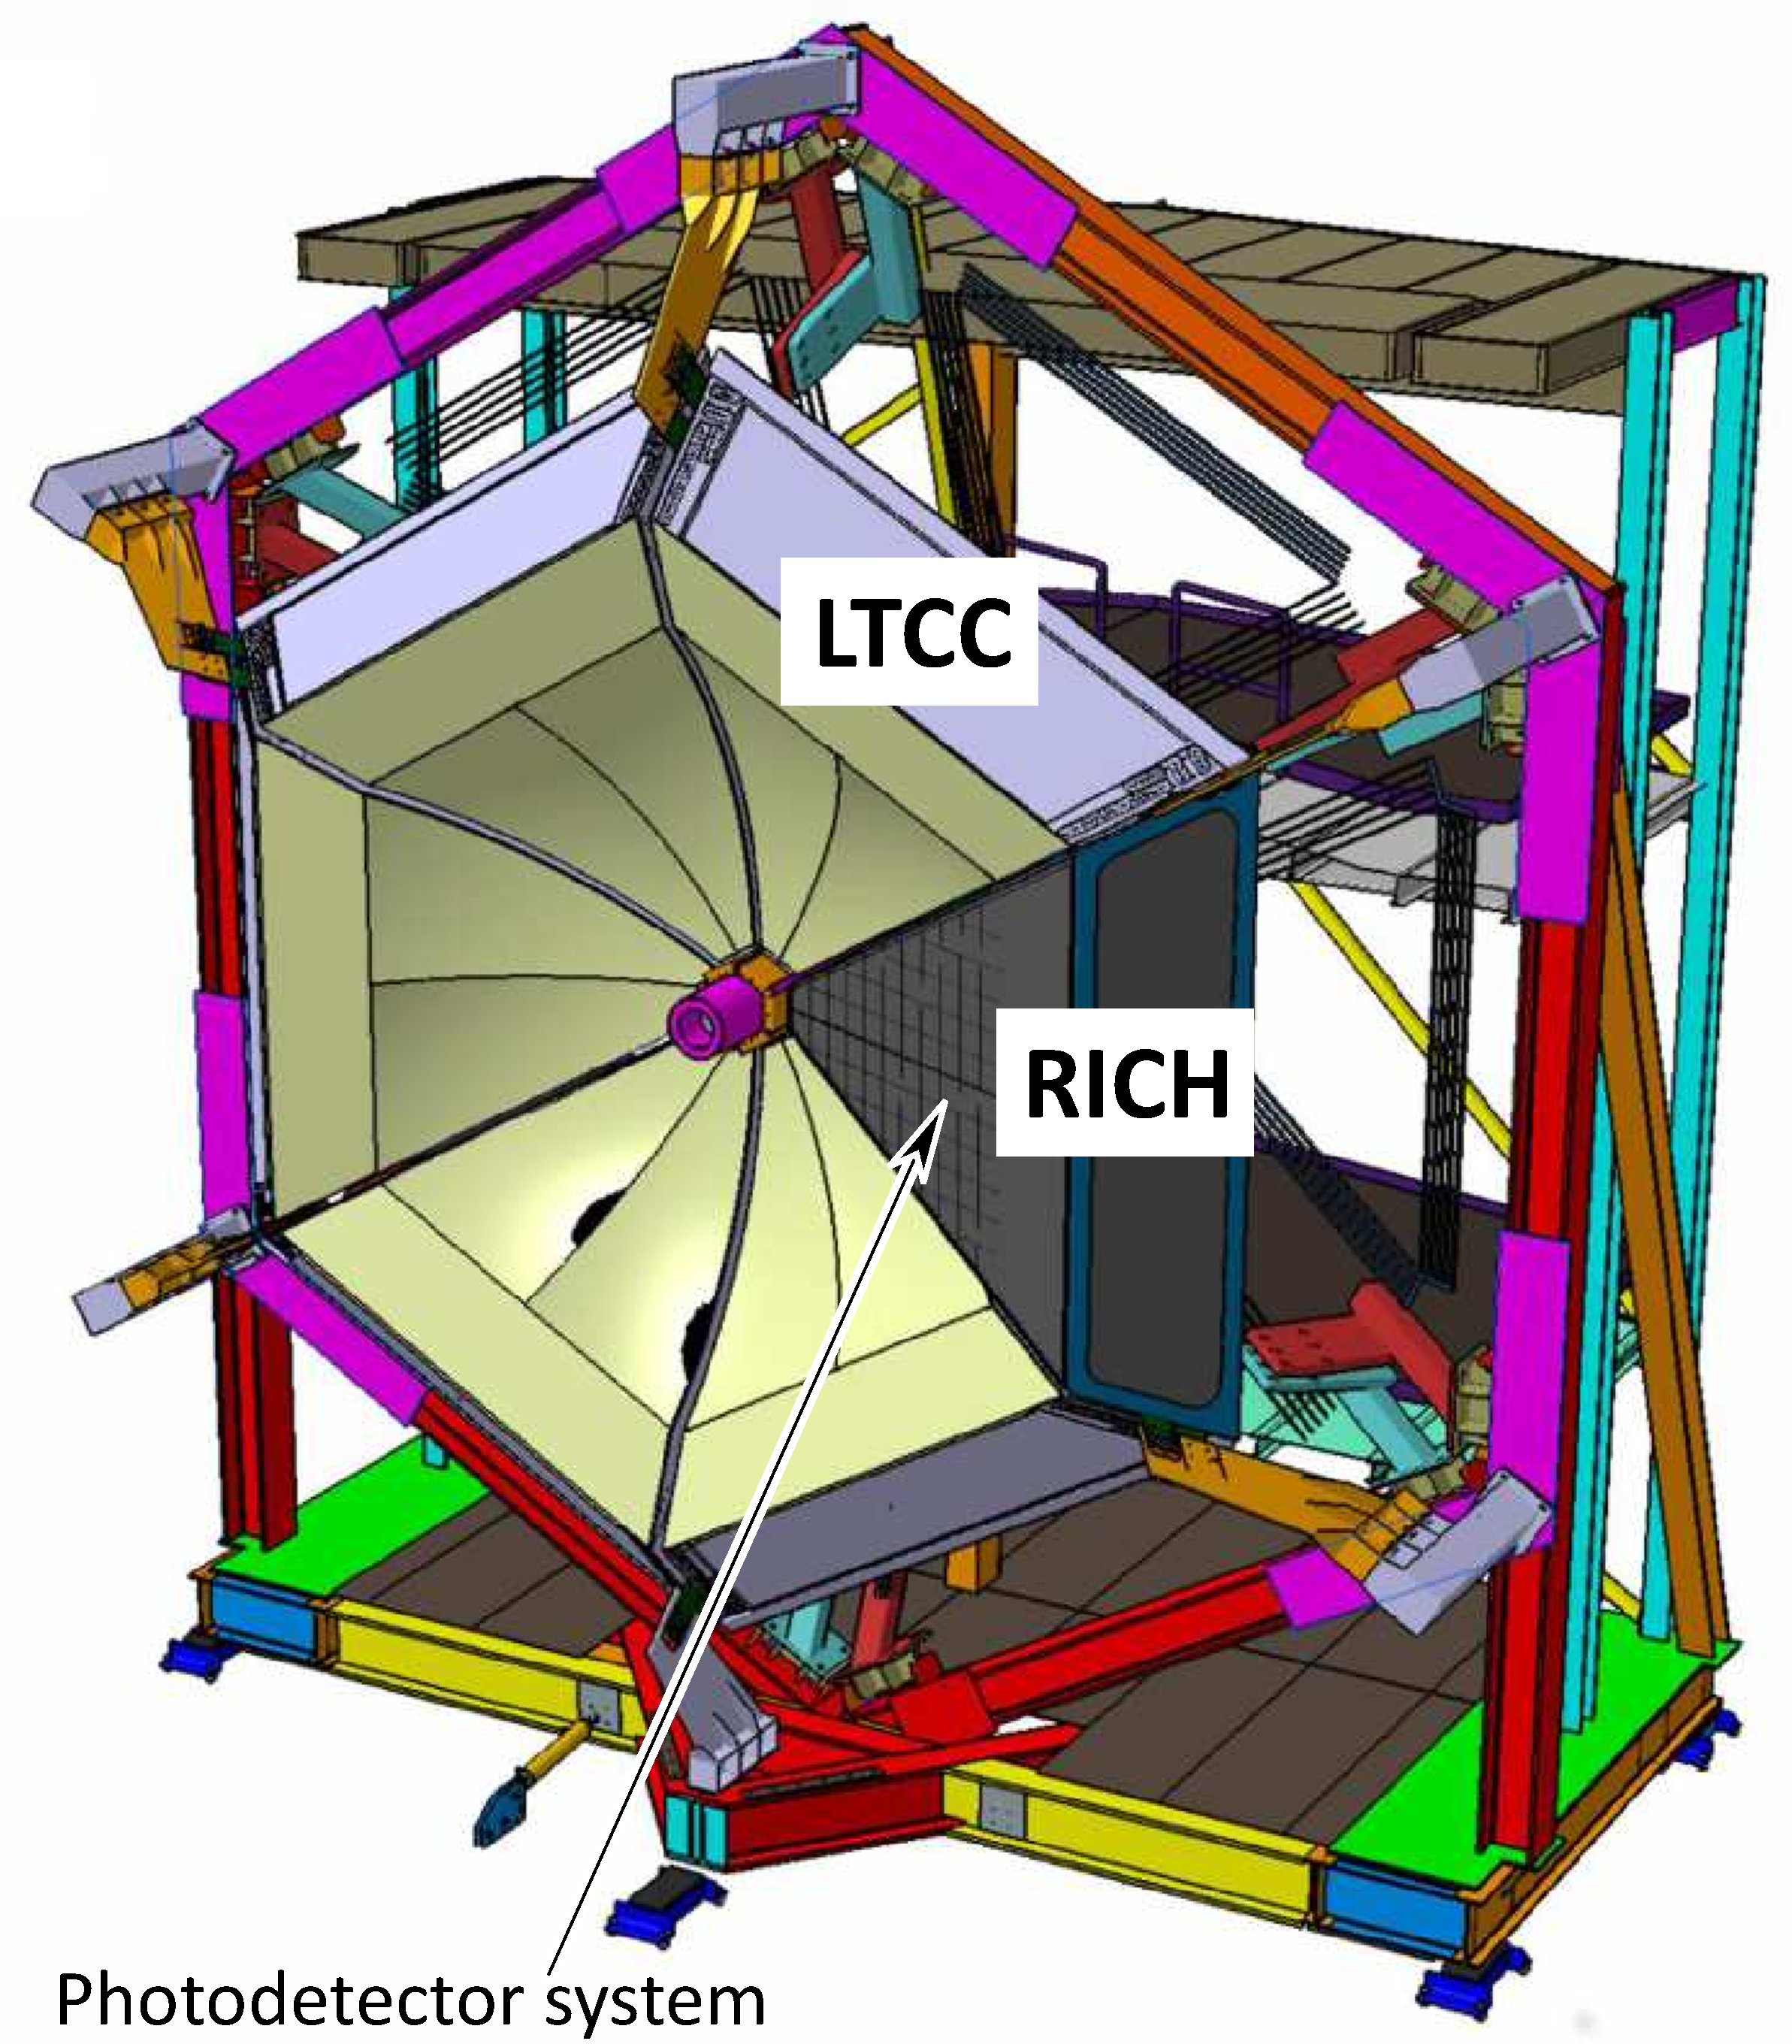
\includegraphics[width=0.95\linewidth]{figures/RICHdetector.pdf}
	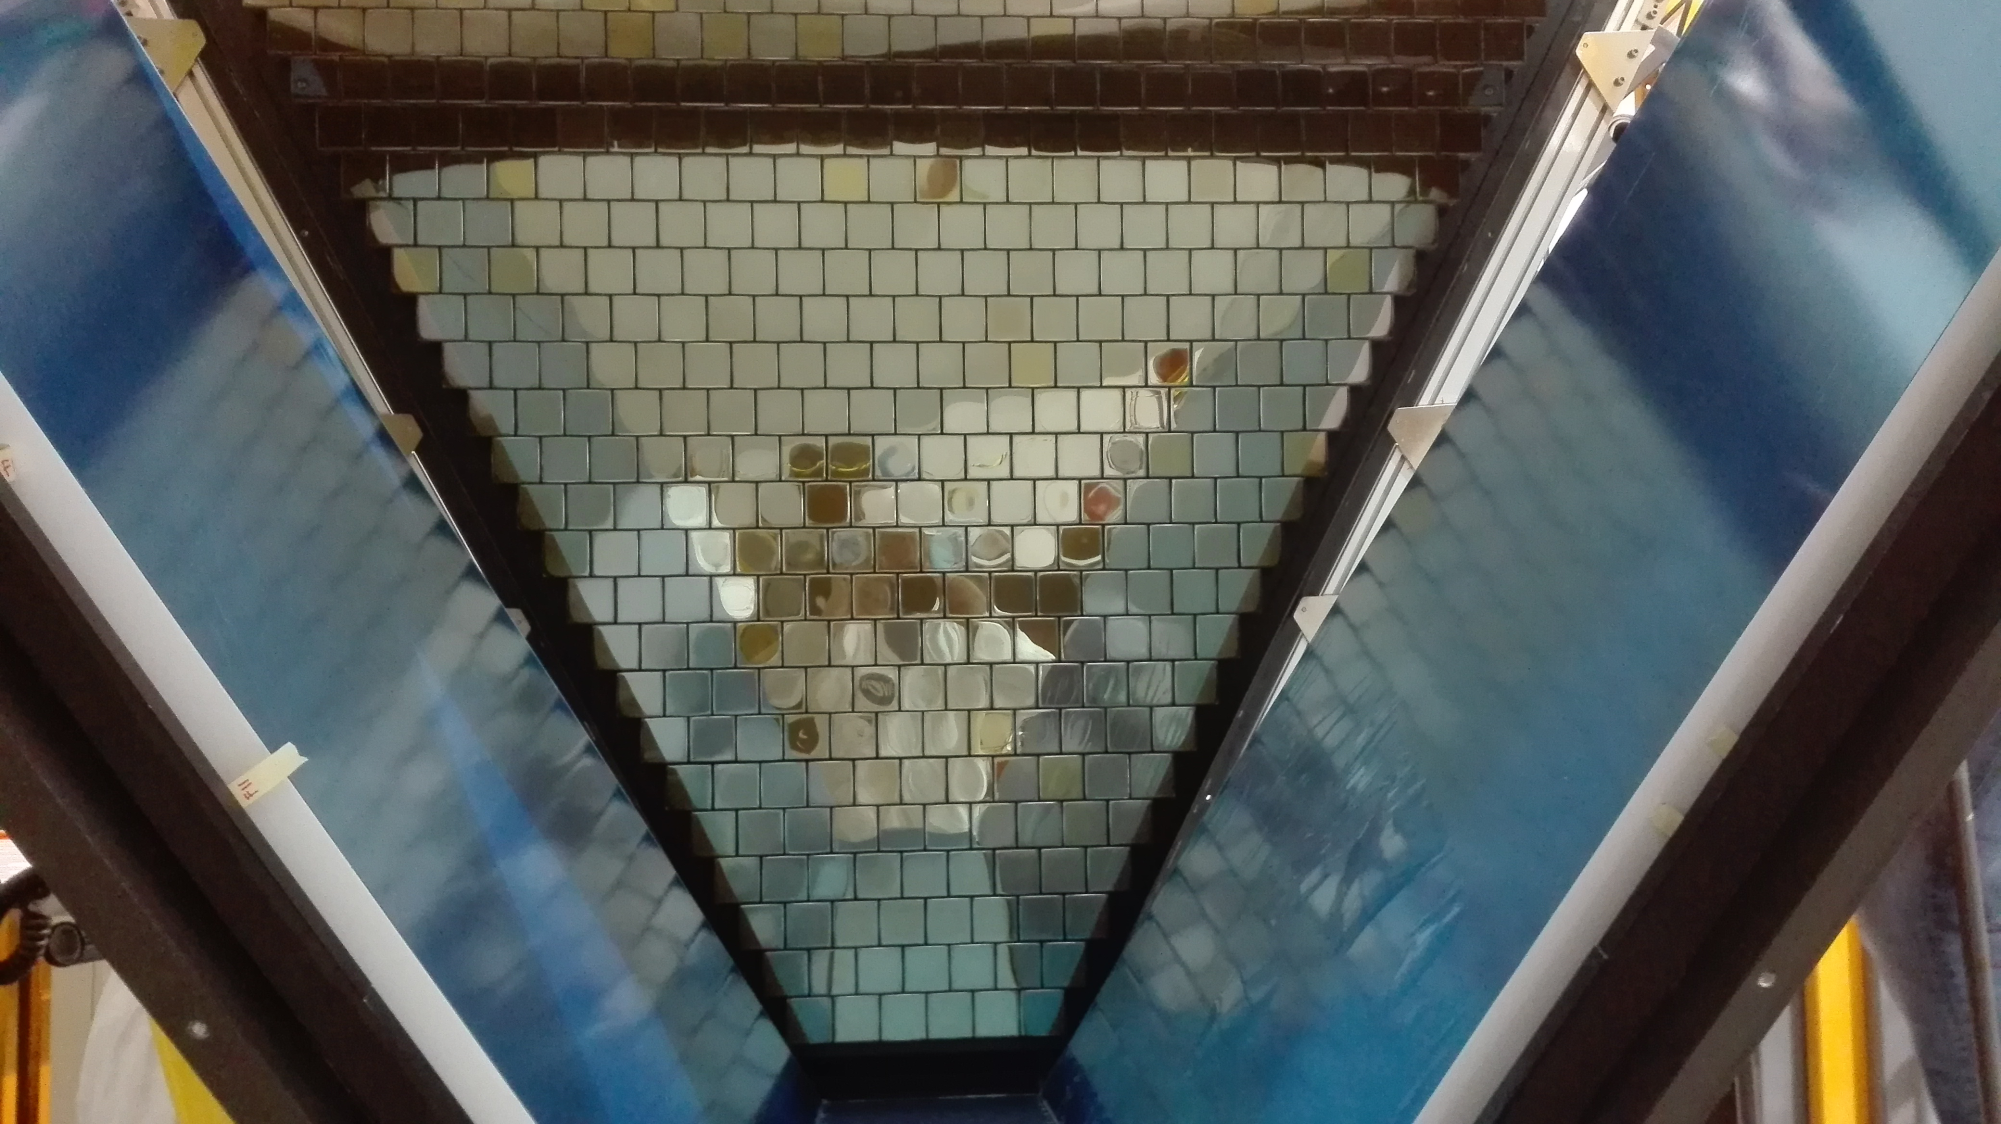
\includegraphics[width=0.95\linewidth]{figures/RICHpanel_front.png}
	\caption{Top: CLAS12 detector with the RICH detector covering one out of six sectors. Bottom: the photomatrix of multianode photomultipliers and the mirror system.}
	\label{fig:RICHdetector}
\end{figure}

The photomatrix  wall is a crucial component of the RICH detector (see Fig.~\ref{fig:RICHdetector}). It is relatively large (area about 1 m$^2$) and should be comprised of many photon detection devices such as photomultiplier tubes.
Due to the imaging aspect of the RICH they must provide a spatial resolution of less than 1 cm.
Since multiple photon detectors are tiled into large arrays, they should have large active area with minimal dead-space.
The photon detectors must also efficiently detect single photon level signals and should be sensitive to visible light due to the aerogel radiator material.
Multianode Photomultiplier Tubes (MAPMTs) from Hamamatsu are perfect candidates for the CLAS12 RICH detector, as they are flat-panel PMTs offering an adequate compromise between detector performance and cost.
Each MAPMT consists of an 8 by 8 array of pixels, each with dimension of 6~mm x 6~mm.
Furthermore, the device has a very high packing fraction of 89\% with a high quantum efficiency in the visible light region.
The tubes also have excellent immunity to magnetic fields, because all internal parts are housed in a metal package and the distance between dynode electrodes is very short.


Initially, the Hamamatsu H8500 MAPMT model \cite{H8500} was chosen as the best option because they provide high quantum efficiency for visible light and sufficient spatial resolution (6x6 mm$^2$) at a limited cost.  However, Hamamatsu has recently released the new H12700 MAPMT model  \cite{H12700} that shows enhanced single photoelectron (SPE) detection, reduced cross-talk between pixels, and is otherwise similar in spatial resolution and  cost to the H8500 
MAPMTs. The first RICH detector was installed in sector 4 of the CLAS12 detector in 2018. There are 391 Hamamatsu MAPMTs  in the photodector matrix, 76 of them are H8500 and 315 H12700. 
The initial characterization of these PMTs was done using a laser stand equipped with a crate of Flash ADC  boards \cite{FADC250} because the custom RICH front-end electronics \cite{RICH_FE} was not ready at that time. The second RICH detector is presently under construction and is planned to be installed in sector 1 of CLAS12 in 2022. The second detector is almost identical to the first one. The characterization of PMTs for this detector was done with standard front-end boards that have much better parameters than the FADCs used in the past. We made detailed characterizations of around 400 H12700 PMTs, as well as several H8500  to make a comparison of the two models. These data give us the possibility to better understand the performance of the first RICH where we are using both PMT models. The results of this study are presented in this paper.



